\documentclass{protokol}
\leftheader{Jednoduché aplikace interference}
\centerheader{Praktikum III}
\rightheader{Tomáš Derner}

\begin{document}

  \section*{Úkol}

    \begin{enumerate}
      \item Změřte tloušťku tenké vrstvy ve dvou různých místech. Vyhodnoťte získané tloušťky a diskutujte, zda je vrstva v rámci chyby nepřímého měření na obou místech stejně silná.
      \item Pomocí Newtonových interferenčních kroužků změřte oba poloměry křivosti u dvou vybraných čoček. Chybu v určení poloměru křivosti stanovte z vhodně použité lineární regrese.
      \item Kontrolu vámi provedené kalibrace stupnice okuláru proveďte metodou postupných měření a zpracujte lineární regresí.
      \item Výsledky měření v bodě 2 porovnejte s optickou mohutností čoček změřenou pomocí fokometru. Index lomu materiálu měřených čoček je \(1,523\).
    \end{enumerate}

  \section*{Teorie}

    \subsection*{Tolanského metoda}

      Pro měření tloušťky tenké vrstvy můžeme využít jevu interference mnoha svazků, přesněji metodu Tolanského. Na měřené vrstvě vytvoříme vryp a vrstvu pokryjeme odrazivým materiálem. Následně mezi takto upravenou vrstvou a polopropustným zrcátkem vytvoříme vzduchovou mezeru s malým úhlem klínu. Toto následně osvětlíme monochromatickým světlem. Interferenční proužky budou v místě vrypu posunuty. V tomto praktiku je již připravená aparatura popsaná detailně v \cite{mereni}. 
      
      Pro tloušťku vrstvy platí vztah
      \begin{equation} \label{eq:vrstva}
        t = \frac{x_1}{x_2} \frac{\lambda}{2},
      \end{equation} 
      kde $x_1$ je posuv polohy interferenčního proužku na vrypu, $x_2$ vzdálenost dvou sousedních proužků a $\lambda$ vlnová délka světla.

    \subsection*{Newtonovy kroužky}

      Osvícením skla položeného na vypuklé čočce získáme obrazec způsobený interferencí na vzduchové vrstvě mezi sklem a čočkou. Tento obrazec sestává ze střídajících se koncentrických světlých a tmavých kroužků. Měřením poloměrů kroužků $\rho_k$ řádů $k$ jsme schopni určit poloměr křivosti čočky $R$ lineární regresí podle vztahu
      \begin{equation} \label{eq:newton}
        \frac{\rho_k^2}{\lambda} = Rk - \frac{Rd}{\lambda},
      \end{equation} 
      kde $d$ je v praxi nenulová vzdálenost čočky od skla.

      Použitá aparatura je opět detailně popsána v \cite{mereni}. Při měření používáme počítačové snímání obrazu z mikroskopu. Tento obraz však musí být kalibrován, protože hodnoty vzdáleností objektů zobrazených mikroskopem samozřejmě závisí na použitém zvětšení. Kalibraci zkontrolujeme metodou postupných měření.
      
      Vypočtené poloměry křivosti čoček ověříme fokometrem. Tento přístroj však měří v optickou mohutnost v jednotkách dioptrie a tato hodnota v sobě zahrnuje křivost obou stran čočky. Optickou mohutnost čočky lze spočíst z indexu lomu prostředí $n$ a poloměrů křivosti $r_1$ a $r_2$ podle vztahu
      \begin{equation} \label{eq:mohutnost}
        \varphi = (n - 1)(\frac{1}{r_1} + \frac{1}{r_2})
      \end{equation}

  \section*{Výsledky}

    Protože s použitými aparaturami nejsme schopni rozlišit individuální vlnové délky sodíkového dubletu $\SI{588.9950}{\nano\metre}$ a $\SI{589.5924}{\nano\metre}$, používáme jejich aritmetický průměr $\lambda = \SI{589.2937}{\nano\metre}$.

    \subsection*{Úkol 1} 
      
      Následující dvě tabulky obsahují naměřené hodnoty potřebné pro výpočet tloušťky tenké vrstvy. Hodnoty $x_{mv}$ a $x_{v}$ jsou odečtené dílky stupnice v polohách proužků mimo vryp a ve vrypu, z nich jsou spočteny hodnoty $x_1$ a $x_2$. Chyba měření byla určena na $\num{0.10}$ dílku.

      \begin{table}[H]
        \centering
        \setlength{\tabcolsep}{10pt}
        \begin{tabular}[t]{
  S[table-format = 1.0]
  S[table-format = 2.2]
  S[table-format = 1.2] 
  S[table-format = 1.2] 
  S[table-format = 1.2] 
} \toprule
{$n$}            & {$x_{mv}$} & {$x_v$} & {$x_1$} & {$x_2$} \\\midrule
1                & 6.37     & 8.22    & 1.85    & 1.08    \\
2                & 5.29     & 7.11    & 1.82    & 1.07    \\
3                & 4.22     & 6.00    & 1.78    & 1.06    \\
4                & 3.16     & 4.94    & 1.78    & 1.07    \\
5                & 2.09     & 3.89    & 1.80    & 1.11    \\
6                & 0.98     & 2.75    & 1.77    & 1.09    \\
7                & -0.11    & 1.67    & 1.78    &         \\\midrule
{\text{průměr}}  &          &         & 1.80    & 1.08    \\
{\text{chyba}}   &          &         & 0.10    & 0.10    \\\bottomrule
\end{tabular}
        \caption{Hodnoty pro první místo vrstvy}
        \label{tab:vrstva1}
      \end{table}
      
      \begin{table}[H]
        \centering
        \setlength{\tabcolsep}{10pt}
        \begin{tabular}[t]{
  S[table-format = 1.0]
  S[table-format = 2.2]
  S[table-format = 1.2] 
  S[table-format = 1.2] 
  S[table-format = 1.2] 
} \toprule
{$n$}            & {$x_{mv}$} & {$x_v$} & {$x_1$} & {$x_2$} \\\midrule
1                & 5.99     & 8.49    & 2.50    & 1.33    \\
2                & 4.66     & 7.04    & 2.38    & 1.39    \\
3                & 3.27     & 5.72    & 2.45    & 1.31    \\
4                & 1.96     & 4.34    & 2.38    & 1.21    \\
5                & 0.75     & 3.03    & 2.28    &         \\\midrule
{\text{průměr}}  &          &         & 2.40    & 1.31    \\
{\text{chyba}}   &          &         & 0.10    & 0.10    \\\bottomrule
\end{tabular}
        \caption{Hodnoty pro druhé místo vrstvy}
        \label{tab:vrstva2}
      \end{table}

      Podle vzorce \eqref{eq:vrstva} byly spočítány tloušťky vrstvy ve dvou místech
      $$ t_1 = \SI{4.9 \pm 0.1 e-7}{\metre}, $$
      $$ t_2 = \SI{5.4 \pm 0.1 e-7}{\metre}. $$
    
    \subsection*{Úkol 2}

      Tabulka \ref{tab:newton} obsahuje naměřené hodnoty poloměrů Newtonových kroužků vytvořených odpovídajícími čočkami. 
      
      \begin{table}[H]
        \centering
        \setlength{\tabcolsep}{10pt}
        \begin{tabular}[t]{
  S[table-format = 2.0] 
  S[table-format = 3.1] 
  S[table-format = 3.1] 
  S[table-format = 3.1] 
  S[table-format = 3.1]
} \toprule
{$k$}            & {$\rho_k^{1A}$}         & {$\rho_k^{1B}$}         & {$\rho_k^{2A}$}         & {$\rho_k^{2B}$}         \\
                 & {$[\si{\micro\metre}]$} & {$[\si{\micro\metre}]$} & {$[\si{\micro\metre}]$} & {$[\si{\micro\metre}]$} \\\midrule
1                & 209.9                   & 213.6                   & 209.9                   & 168.3                   \\
2                & 295                     & 305.9                   & 316.7                   & 238.9                   \\
3                & 360.2                   & 372.8                   & 398.2                   & 291.4                   \\
4                & 416.3                   & 430.7                   & 463.3                   & 338.4                   \\
5                & 465.1                   & 483.2                   & 523.1                   & 376.5                   \\
6                & 510.4                   & 528.5                   & 575.5                   & 412.7                   \\
7                & 550.2                   & 571.9                   & 622.6                   & 445.2                   \\
8                & 590                     & 611.7                   & 666                     & 476                     \\
9                & 624.4                   & 647.9                   & 707.7                   & 506.8                   \\
10               & 660.6                   & 682.3                   & 749.3                   & 532.1                   \\\bottomrule
  \end{tabular}
        \caption{Poloměry Newtonových kroužků pro dvě čočky z obou stran}
        \label{tab:newton}
      \end{table}

      Následující graf zachycuje použité lineární regrese podle vztahu \eqref{eq:newton}.
      
      \begin{figure}[H]
        \centering
        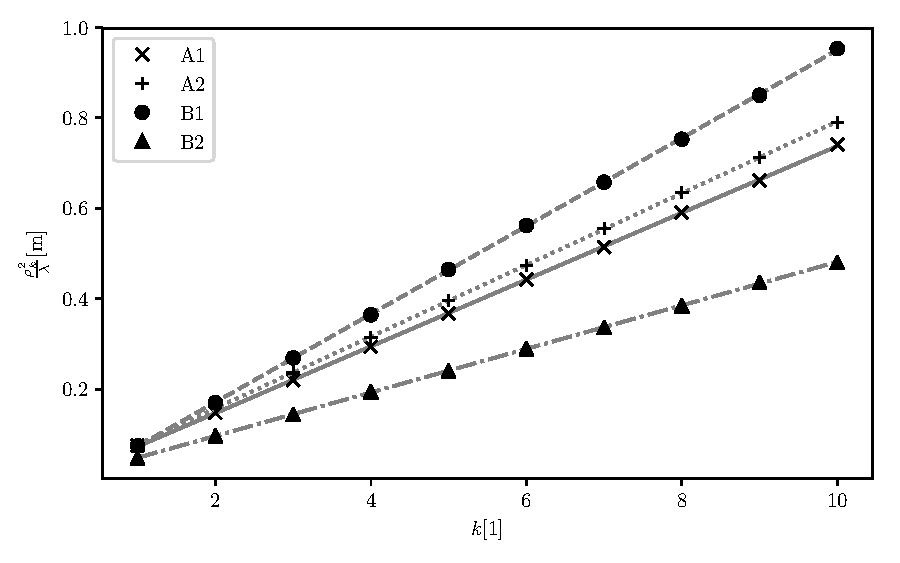
\includegraphics[]{newton}
        \caption{Lineární závislosti použité k získání poloměrů křivosti}
        \label{fig:newton}
      \end{figure}

      Byly získány hodnoty poloměrů křivosti
      $$ R_{A1} = \SI{0.073 \pm 0.001}{m}, $$
      $$ R_{A2} = \SI{0.079 \pm 0.001}{m}, $$
      $$ R_{B1} = \SI{0.097 \pm 0.001}{m}, $$
      $$ R_{B2} = \SI{0.048 \pm 0.001}{m}. $$

      Chyby hodnot odpovídají chybám regrese.

    \subsection*{Úkol 3}
      
      Před začátkem měření Newtonových kroužků byla provedena kalibrace použitého softwarového systému a následně její ověření pomocí metody postupných měření. Regresí získaných hodnot jsme dostali směrnici (tedy poměr skutečné a zobrazené hodnoty) $\SI{1.0007 \pm 0.0006}{}$, chybu kalibrace tedy považujeme za nepodstatnou. 

      \begin{figure}[H]
        \centering
        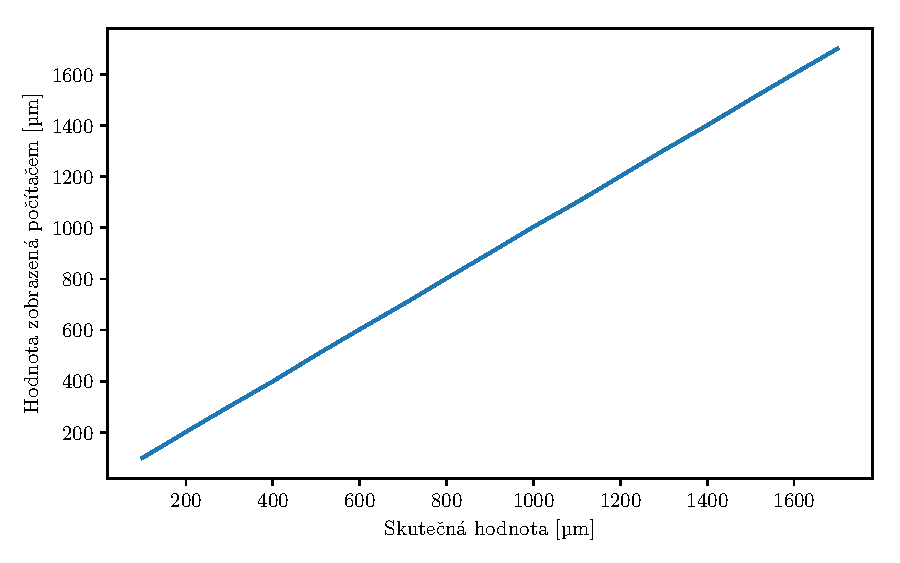
\includegraphics[]{kalibrace}
        \caption{Kalibrace softwarového systému použitého k měření}
        \label{fig:u4s}
      \end{figure}

    \subsection*{Úkol 4}

      Fokometrem byla změřena optická mohutnost čoček 
      $$ \varphi_A = \SI{13.75 \pm 0.25}{D}, $$
      $$ \varphi_B = \SI{17.25 \pm 0.25}{D}. $$

      Z předchozích výsledků byly podle vztahu \eqref{eq:mohutnost} spočteny optické mohutnosti
      $$ \varphi_A = \SI{13.78 \pm 0.13}{D}, $$
      $$ \varphi_B = \SI{16.29 \pm 0.23}{D}. $$

  \section*{Diskuse}

    Při měření tloušťky vrstvy byly polohy interferenčních proužků měřeny v místě přechodu světlého a tmavého proužku. Interferenční obrazec byl však značně rozmazaný, tedy nebylo snadné rozeznat přesnou hranici proužku, a proto byla naměřeným hodnotám přiřčena značná chyba. I přes to je však zřejmé, že tloušťka vrstvy se v měřených místech značně liší.

    Hodnota optické mohutnosti čočky A spočtená z poloměrů křivosti získaných pomocí Newtonových kroužků se moc neliší a toto měření se dá považovat za úspěšné. Hodnoty pro čočku B se však od sebe liší o zhruba dvojnásobek součtu chyb, v průběhu měření tedy vznikla značná chyba, nejspíše hrubého druhu.

  \section*{Závěr}

    Byla změřena tloušťka tenké vrstvy na dvou místech 
    $$ t_1 = \SI{4.9 \pm 0.1 e-7}{\metre}, $$
    $$ t_2 = \SI{5.4 \pm 0.1 e-7}{\metre}. $$

    Byly změřeny poloměry křivosti dvou čoček 
    $$ R_{A1} = \SI{0.073 \pm 0.001}{m}, $$
    $$ R_{A2} = \SI{0.079 \pm 0.001}{m}, $$
    $$ R_{B1} = \SI{0.097 \pm 0.001}{m}, $$
    $$ R_{B2} = \SI{0.048 \pm 0.001}{m}. $$

    Z ověření kalibrace metodou postupných měření vyplynula zanedbatelná chyba kalibrace.

    Fokometrem byla změřena optická mohutnost čoček 
    $$ \varphi_A = \SI{13.75 \pm 0.25}{D}, $$
    $$ \varphi_B = \SI{17.25 \pm 0.25}{D}, $$
    hodnoty spočtené pomocí Newtonových kroužků jsou
    $$ \varphi_A = \SI{13.78 \pm 0.13}{D}, $$
    $$ \varphi_B = \SI{16.29 \pm 0.23}{D}. $$
    
  \begin{thebibliography}{}

    \bibitem{mereni}
    Pokyny k měření "Jednoduché aplikace interferenčních jevů", dostupné z\\ \url{http://physics.mff.cuni.cz/vyuka/zfp/_media/zadani/pokyny/mereni_330.pdf}, 3.\,3.\,2018
  
  \end{thebibliography}

\end{document}